\section{dg::Visualizer Class Reference}
\label{classdg_1_1Visualizer}\index{dg::Visualizer@{dg::Visualizer}}
{\tt \#include $<$Visualizer.h$>$}

Inheritance diagram for dg::Visualizer:\begin{figure}[H]
\begin{center}
\leavevmode
\includegraphics[width=55pt]{classdg_1_1Visualizer__inherit__graph}
\end{center}
\end{figure}
Collaboration diagram for dg::Visualizer:\begin{figure}[H]
\begin{center}
\leavevmode
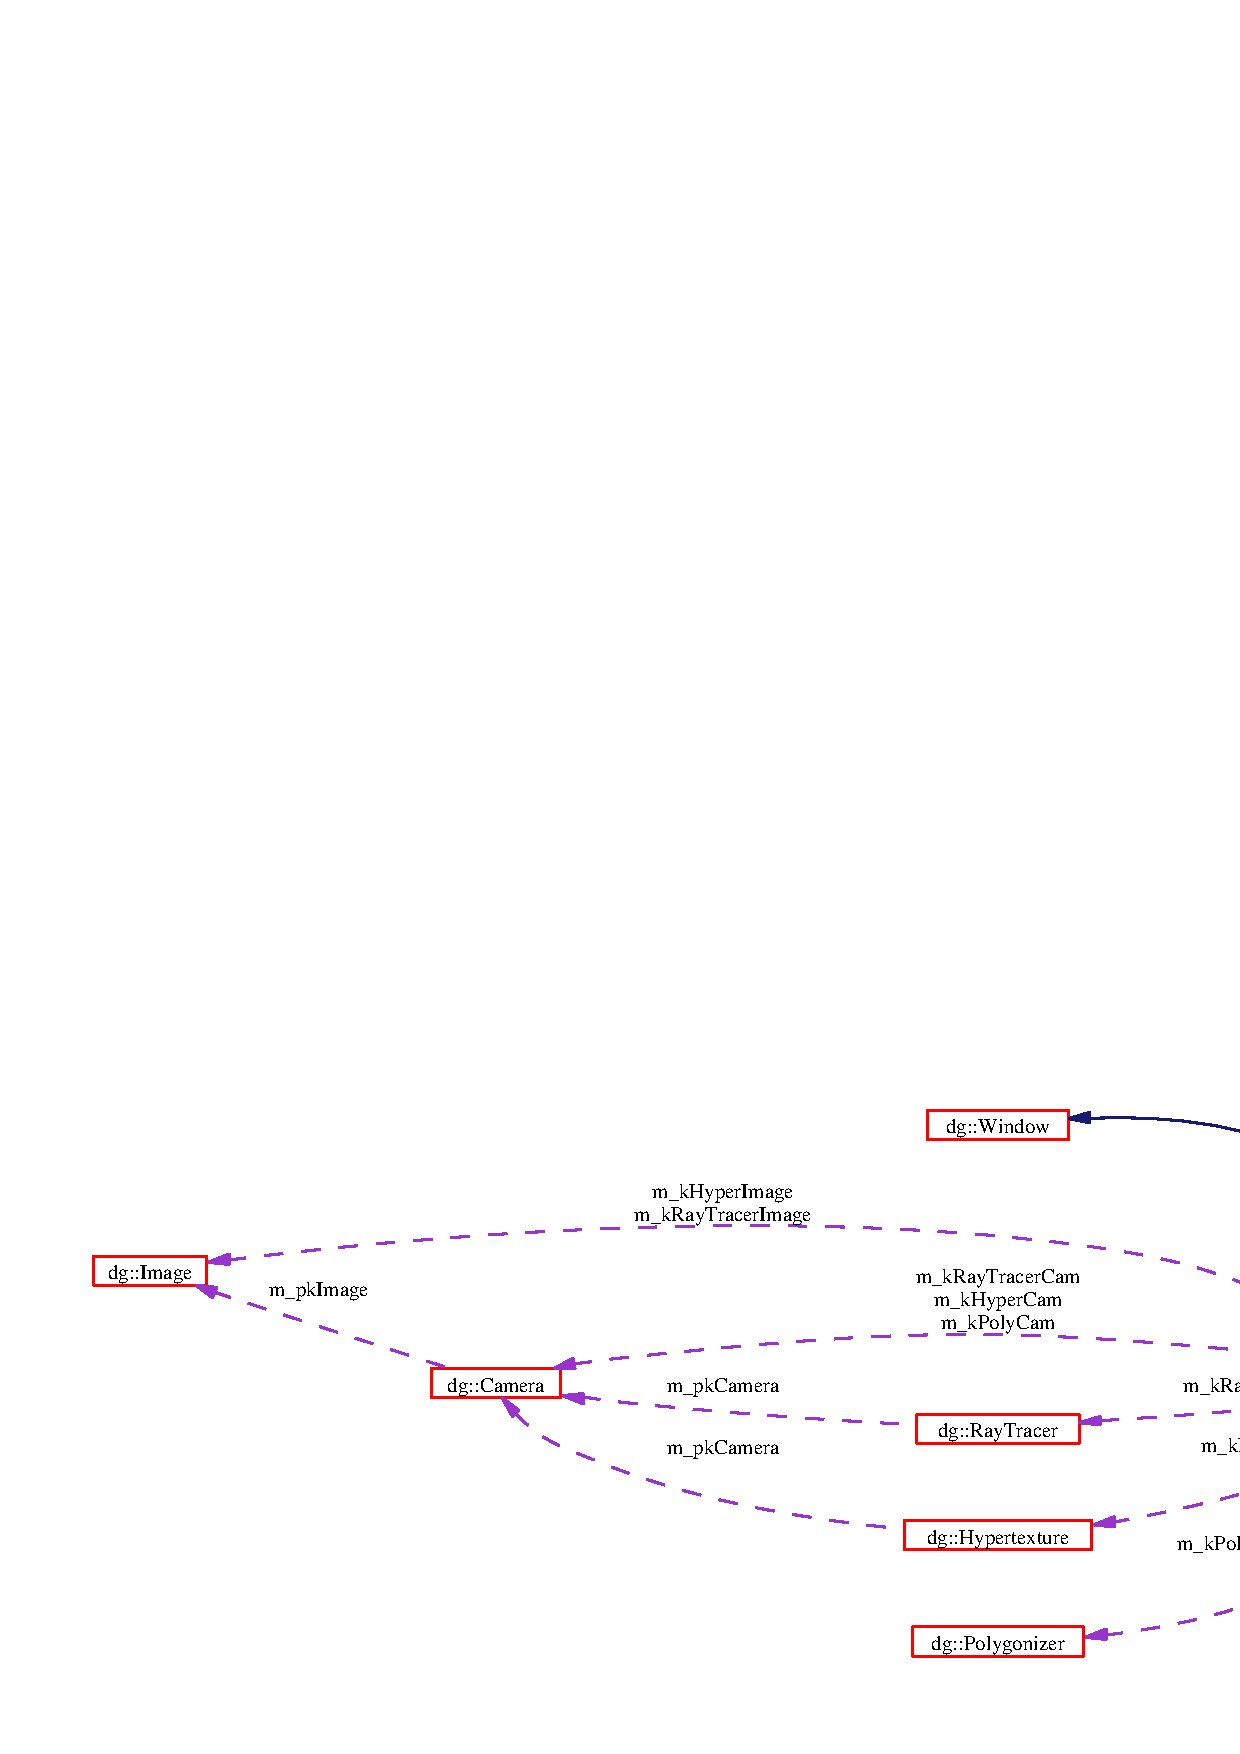
\includegraphics[width=372pt]{classdg_1_1Visualizer__coll__graph}
\end{center}
\end{figure}
\subsection*{Public Types}
\begin{CompactItemize}
\item 
enum {\bf Visualizer\-Mode} \{ {\bf VM\_\-MARCHING\_\-CUBES}, 
{\bf VM\_\-MARCHING\_\-TETRA}, 
{\bf VM\_\-RAYTRACE}, 
{\bf VM\_\-HYPERTEXTURE}, 
{\bf VM\_\-COUNT}
 \}
\end{CompactItemize}
\subsection*{Public Methods}
\begin{CompactItemize}
\item 
{\bf Visualizer} ()
\item 
virtual {\bf $\sim$Visualizer} ()
\item 
virtual {\bf Bool} {\bf on\-Startup} ()
\item 
virtual {\bf Bool} {\bf on\-Initialize} ()
\item 
virtual void {\bf on\-Reshape} ({\bf Int} i\-Width, {\bf Int} i\-Height)
\item 
virtual void {\bf on\-Display} ()
\item 
virtual void {\bf on\-Idle} ()
\item 
virtual void {\bf on\-Key\-Down} ({\bf UChar} uc\-Key, {\bf Int} i\-X, {\bf Int} i\-Y)
\item 
virtual void {\bf on\-Special\-Key\-Down} ({\bf Int} i\-Key, {\bf Int} i\-X, {\bf Int} i\-Y)
\item 
virtual void {\bf on\-Mouse\-Motion} ({\bf Int} i\-X, {\bf Int} i\-Y, {\bf UInt} ui\-Modifiers)
\item 
virtual void {\bf on\-Mouse\-Click} ({\bf Int} i\-Button, {\bf Int} i\-State, {\bf Int} i\-X, {\bf Int} i\-Y, {\bf UInt} ui\-Modifiers)
\item 
void {\bf draw\-Text} ()
\item 
void {\bf draw\-Polygons} ()
\item 
void {\bf draw\-Raytraced} ()
\item 
void {\bf draw\-Hypertexture} ()
\end{CompactItemize}
\subsection*{Protected Methods}
\begin{CompactItemize}
\item 
void {\bf setup\-Polygonizer} ()
\item 
void {\bf setup\-Ray\-Tracer} ()
\item 
void {\bf setup\-Hypertexture} ()
\item 
void {\bf setup\-Camera} ({\bf Camera} \&rk\-Camera)
\item 
void {\bf setup\-Frustum} ({\bf Int} i\-Width, {\bf Int} i\-Height, bool b\-Perspective)
\item 
void {\bf set\-Background} ()
\item 
void {\bf set\-Lights} ()
\item 
void {\bf set\-Materials} ()
\item 
void {\bf start\-Calc\-Timer} ()
\item 
void {\bf update\-Calc\-Timer} ()
\item 
void {\bf stop\-Calc\-Timer} ()
\item 
void {\bf update} ({\bf Real} f\-Time)
\end{CompactItemize}
\subsection*{Protected Attributes}
\begin{CompactItemize}
\item 
{\bf Real} {\bf m\_\-f\-Last\-Calc\-Time}
\item 
{\bf UInt} {\bf m\_\-ui\-Hours}
\item 
{\bf UInt} {\bf m\_\-ui\-Minutes}
\item 
{\bf UInt} {\bf m\_\-ui\-Seconds}
\item 
{\bf UInt} {\bf m\_\-ui\-Milli\-Secs}
\item 
bool {\bf m\_\-b\-Use\-Perspective}
\item 
bool {\bf m\_\-b\-Show\-Info}
\item 
bool {\bf m\_\-b\-Update}
\item 
bool {\bf m\_\-b\-Rotate}
\item 
bool {\bf m\_\-b\-Show\-Bounds}
\item 
bool {\bf m\_\-b\-Spin}
\item 
bool {\bf m\_\-b\-Move}
\item 
bool {\bf m\_\-b\-Light}
\item 
bool {\bf m\_\-b\-Rendering}
\item 
bool {\bf m\_\-b\-Ray\-Traced}
\item 
bool {\bf m\_\-b\-Hyper\-Traced}
\item 
bool {\bf m\_\-b\-Polygonized}
\item 
bool {\bf m\_\-b\-Keep\-In\-View}
\item 
bool {\bf m\_\-b\-Fade\-Out}
\item 
{\bf Int} {\bf m\_\-i\-Spin\-X}
\item 
{\bf Int} {\bf m\_\-i\-Spin\-Y}
\item 
{\bf Int} {\bf m\_\-i\-Orig\-X}
\item 
{\bf Int} {\bf m\_\-i\-Orig\-Y}
\item 
{\bf Int} {\bf m\_\-i\-Cell\-Count}
\item 
{\bf Real} {\bf m\_\-f\-Scale}
\item 
{\bf Real} {\bf m\_\-f\-Iso\-Level}
\item 
{\bf Real} {\bf m\_\-f\-Update\-Offset}
\item 
{\bf Real} {\bf m\_\-f\-Time}
\item 
{\bf Polygonizer::March\-Method} {\bf m\_\-e\-March\-Mode}
\item 
{\bf Real} {\bf m\_\-f\-Transparency}
\item 
{\bf Real} {\bf m\_\-f\-Offset\-X}
\item 
{\bf Real} {\bf m\_\-f\-Offset\-Y}
\item 
{\bf Real} {\bf m\_\-f\-Offset\-Z}
\item 
{\bf Real} {\bf m\_\-f\-Camera\-X}
\item 
{\bf Real} {\bf m\_\-f\-Camera\-Y}
\item 
{\bf Real} {\bf m\_\-f\-Camera\-Z}
\item 
{\bf Real} {\bf m\_\-f\-Frustum\-Left}
\item 
{\bf Real} {\bf m\_\-f\-Frustum\-Right}
\item 
{\bf Real} {\bf m\_\-f\-Frustum\-Bottom}
\item 
{\bf Real} {\bf m\_\-f\-Frustum\-Top}
\item 
{\bf Real} {\bf m\_\-f\-Frustum\-Near}
\item 
{\bf Real} {\bf m\_\-f\-Frustum\-Far}
\item 
{\bf Int} {\bf m\_\-e\-Poly\-Mode}
\item 
{\bf Polygonizer} {\bf m\_\-k\-Polygonizer}
\item 
{\bf Camera} {\bf m\_\-k\-Poly\-Cam}
\item 
{\bf Ray\-Tracer} {\bf m\_\-k\-Ray\-Tracer}
\item 
{\bf Camera} {\bf m\_\-k\-Ray\-Tracer\-Cam}
\item 
{\bf Image} {\bf m\_\-k\-Ray\-Tracer\-Image}
\item 
{\bf Hypertexture} {\bf m\_\-k\-Hyper}
\item 
{\bf Camera} {\bf m\_\-k\-Hyper\-Cam}
\item 
{\bf Image} {\bf m\_\-k\-Hyper\-Image}
\item 
{\bf UInt} {\bf m\_\-ui\-Func\-Index}
\item 
const char $\ast$ {\bf m\_\-auc\-Func\-Name}
\item 
{\bf Operator} {\bf m\_\-pv\-Function}
\item 
{\bf Visualizer\-Mode} {\bf m\_\-e\-Vis\-Mode}
\end{CompactItemize}
\subsection*{Static Protected Attributes}
\begin{CompactItemize}
\item 
const {\bf Real} {\bf ms\_\-f\-Cell\-To\-Ray\-Scale} = 2
\item 
const {\bf Real} {\bf ms\_\-f\-Cell\-To\-Hyper\-Step\-Scale} = 0.4
\end{CompactItemize}


\subsection{Member Enumeration Documentation}
\index{dg::Visualizer@{dg::Visualizer}!VisualizerMode@{VisualizerMode}}
\index{VisualizerMode@{VisualizerMode}!dg::Visualizer@{dg::Visualizer}}
\subsubsection{\setlength{\rightskip}{0pt plus 5cm}enum dg::Visualizer::Visualizer\-Mode}\label{classdg_1_1Visualizer_s5}


\begin{Desc}
\item[Enumeration values: ]\par
\begin{description}
\index{VM_MARCHING_CUBES@{VM\_\-MARCHING\_\-CUBES}!dg::Visualizer@{dg::Visualizer}}\index{dg::Visualizer@{dg::Visualizer}!VM_MARCHING_CUBES@{VM\_\-MARCHING\_\-CUBES}}\item[{\em 
{\em VM\_\-MARCHING\_\-CUBES}\label{classdg_1_1Visualizer_s5s0}
}]\index{VM_MARCHING_TETRA@{VM\_\-MARCHING\_\-TETRA}!dg::Visualizer@{dg::Visualizer}}\index{dg::Visualizer@{dg::Visualizer}!VM_MARCHING_TETRA@{VM\_\-MARCHING\_\-TETRA}}\item[{\em 
{\em VM\_\-MARCHING\_\-TETRA}\label{classdg_1_1Visualizer_s5s1}
}]\index{VM_RAYTRACE@{VM\_\-RAYTRACE}!dg::Visualizer@{dg::Visualizer}}\index{dg::Visualizer@{dg::Visualizer}!VM_RAYTRACE@{VM\_\-RAYTRACE}}\item[{\em 
{\em VM\_\-RAYTRACE}\label{classdg_1_1Visualizer_s5s2}
}]\index{VM_HYPERTEXTURE@{VM\_\-HYPERTEXTURE}!dg::Visualizer@{dg::Visualizer}}\index{dg::Visualizer@{dg::Visualizer}!VM_HYPERTEXTURE@{VM\_\-HYPERTEXTURE}}\item[{\em 
{\em VM\_\-HYPERTEXTURE}\label{classdg_1_1Visualizer_s5s3}
}]\index{VM_COUNT@{VM\_\-COUNT}!dg::Visualizer@{dg::Visualizer}}\index{dg::Visualizer@{dg::Visualizer}!VM_COUNT@{VM\_\-COUNT}}\item[{\em 
{\em VM\_\-COUNT}\label{classdg_1_1Visualizer_s5s4}
}]\end{description}
\end{Desc}



Definition at line 22 of file Visualizer.h.

\subsection{Constructor \& Destructor Documentation}
\index{dg::Visualizer@{dg::Visualizer}!Visualizer@{Visualizer}}
\index{Visualizer@{Visualizer}!dg::Visualizer@{dg::Visualizer}}
\subsubsection{\setlength{\rightskip}{0pt plus 5cm}Visualizer::Visualizer ()}\label{classdg_1_1Visualizer_a0}




Definition at line 16 of file Visualizer.cpp.\index{dg::Visualizer@{dg::Visualizer}!~Visualizer@{$\sim$Visualizer}}
\index{~Visualizer@{$\sim$Visualizer}!dg::Visualizer@{dg::Visualizer}}
\subsubsection{\setlength{\rightskip}{0pt plus 5cm}Visualizer::$\sim$Visualizer ()\hspace{0.3cm}{\tt  [virtual]}}\label{classdg_1_1Visualizer_a1}




Definition at line 23 of file Visualizer.cpp.

\subsection{Member Function Documentation}
\index{dg::Visualizer@{dg::Visualizer}!drawHypertexture@{drawHypertexture}}
\index{drawHypertexture@{drawHypertexture}!dg::Visualizer@{dg::Visualizer}}
\subsubsection{\setlength{\rightskip}{0pt plus 5cm}void Visualizer::draw\-Hypertexture ()}\label{classdg_1_1Visualizer_a14}




Definition at line 210 of file Visualizer.cpp.

References dg::Window::draw\-Image(), draw\-Text(), dg::Image::height(), m\_\-b\-Hyper\-Traced, m\_\-b\-Rendering, m\_\-b\-Update, m\_\-k\-Hyper, m\_\-k\-Hyper\-Image, dg::Image::pixels(), dg::Window::post\-Redisplay(), dg::Hypertexture::render(), set\-Background(), start\-Calc\-Timer(), stop\-Calc\-Timer(), dg::Window::swap\-Buffers(), dg::UInt, update\-Calc\-Timer(), and dg::Image::width().

Referenced by on\-Display().\index{dg::Visualizer@{dg::Visualizer}!drawPolygons@{drawPolygons}}
\index{drawPolygons@{drawPolygons}!dg::Visualizer@{dg::Visualizer}}
\subsubsection{\setlength{\rightskip}{0pt plus 5cm}void Visualizer::draw\-Polygons ()}\label{classdg_1_1Visualizer_a12}




Definition at line 269 of file Visualizer.cpp.

References dg::Polygonizer::evaluate(), dg::Polygonizer::get\-Colors(), dg::Camera::get\-Direction(), dg::Polygonizer::get\-Normals(), dg::Camera::get\-Position(), dg::Camera::get\-Up(), dg::Polygonizer::get\-Vertices(), m\_\-b\-Light, m\_\-b\-Polygonized, m\_\-b\-Update, m\_\-e\-March\-Mode, m\_\-k\-Poly\-Cam, m\_\-k\-Polygonizer, setup\-Camera(), start\-Calc\-Timer(), stop\-Calc\-Timer(), dg::UInt, dg::Vector::x(), dg::Vector::y(), and dg::Vector::z().

Referenced by on\-Display().\index{dg::Visualizer@{dg::Visualizer}!drawRaytraced@{drawRaytraced}}
\index{drawRaytraced@{drawRaytraced}!dg::Visualizer@{dg::Visualizer}}
\subsubsection{\setlength{\rightskip}{0pt plus 5cm}void Visualizer::draw\-Raytraced ()}\label{classdg_1_1Visualizer_a13}




Definition at line 151 of file Visualizer.cpp.

References dg::Window::draw\-Image(), draw\-Text(), dg::Image::height(), m\_\-b\-Ray\-Traced, m\_\-b\-Rendering, m\_\-b\-Update, m\_\-k\-Ray\-Tracer, m\_\-k\-Ray\-Tracer\-Image, dg::Image::pixels(), dg::Window::post\-Redisplay(), dg::Ray\-Tracer::render(), set\-Background(), start\-Calc\-Timer(), stop\-Calc\-Timer(), dg::Window::swap\-Buffers(), dg::UInt, update\-Calc\-Timer(), and dg::Image::width().

Referenced by on\-Display().\index{dg::Visualizer@{dg::Visualizer}!drawText@{drawText}}
\index{drawText@{drawText}!dg::Visualizer@{dg::Visualizer}}
\subsubsection{\setlength{\rightskip}{0pt plus 5cm}void Visualizer::draw\-Text ()}\label{classdg_1_1Visualizer_a11}




Definition at line 336 of file Visualizer.cpp.

References dg::Color::a(), dg::Color::b(), dg::Char, dg::Window::draw\-String(), dg::Color::g(), dg::Hypertexture::get\-Ray\-Hits(), dg::Ray\-Tracer::get\-Ray\-Hits(), dg::Hypertexture::get\-Samples(), dg::Hypertexture::get\-Step\-Size(), dg::Polygonizer::get\-Vertices(), dg::Window::height(), dg::Int, m\_\-auc\-Func\-Name, m\_\-e\-Vis\-Mode, m\_\-f\-Iso\-Level, m\_\-f\-Offset\-X, m\_\-f\-Offset\-Y, m\_\-f\-Offset\-Z, m\_\-f\-Scale, m\_\-i\-Cell\-Count, m\_\-i\-Spin\-X, m\_\-i\-Spin\-Y, m\_\-k\-Hyper, m\_\-k\-Polygonizer, m\_\-k\-Ray\-Tracer, m\_\-ui\-Hours, m\_\-ui\-Milli\-Secs, m\_\-ui\-Minutes, m\_\-ui\-Seconds, ms\_\-f\-Cell\-To\-Ray\-Scale, dg::Color::r(), dg::UInt, VM\_\-HYPERTEXTURE, VM\_\-MARCHING\_\-CUBES, VM\_\-MARCHING\_\-TETRA, VM\_\-RAYTRACE, and dg::Window::width().

Referenced by draw\-Hypertexture(), draw\-Raytraced(), and on\-Display().\index{dg::Visualizer@{dg::Visualizer}!onDisplay@{onDisplay}}
\index{onDisplay@{onDisplay}!dg::Visualizer@{dg::Visualizer}}
\subsubsection{\setlength{\rightskip}{0pt plus 5cm}void Visualizer::on\-Display ()\hspace{0.3cm}{\tt  [virtual]}}\label{classdg_1_1Visualizer_a5}




Reimplemented from {\bf dg::Window} {\rm (p.\,\pageref{classdg_1_1Window_a7})}.

Definition at line 125 of file Visualizer.cpp.

References draw\-Hypertexture(), draw\-Polygons(), draw\-Raytraced(), draw\-Text(), m\_\-b\-Update, m\_\-e\-Vis\-Mode, m\_\-f\-Time, dg::Window::swap\-Buffers(), update(), dg::Window::update\-Clicks(), VM\_\-HYPERTEXTURE, VM\_\-MARCHING\_\-CUBES, VM\_\-MARCHING\_\-TETRA, and VM\_\-RAYTRACE.

Referenced by on\-Idle().\index{dg::Visualizer@{dg::Visualizer}!onIdle@{onIdle}}
\index{onIdle@{onIdle}!dg::Visualizer@{dg::Visualizer}}
\subsubsection{\setlength{\rightskip}{0pt plus 5cm}virtual void dg::Visualizer::on\-Idle ()\hspace{0.3cm}{\tt  [inline, virtual]}}\label{classdg_1_1Visualizer_a6}




Reimplemented from {\bf dg::Window} {\rm (p.\,\pageref{classdg_1_1Window_a17})}.

Definition at line 41 of file Visualizer.h.

References on\-Display().\index{dg::Visualizer@{dg::Visualizer}!onInitialize@{onInitialize}}
\index{onInitialize@{onInitialize}!dg::Visualizer@{dg::Visualizer}}
\subsubsection{\setlength{\rightskip}{0pt plus 5cm}{\bf Bool} Visualizer::on\-Initialize ()\hspace{0.3cm}{\tt  [virtual]}}\label{classdg_1_1Visualizer_a3}




Reimplemented from {\bf dg::Window} {\rm (p.\,\pageref{classdg_1_1Window_a2})}.

Definition at line 85 of file Visualizer.cpp.

References dg::Bool, dg::Window::height(), on\-Reshape(), set\-Background(), set\-Lights(), set\-Materials(), setup\-Polygonizer(), and dg::Window::width().\index{dg::Visualizer@{dg::Visualizer}!onKeyDown@{onKeyDown}}
\index{onKeyDown@{onKeyDown}!dg::Visualizer@{dg::Visualizer}}
\subsubsection{\setlength{\rightskip}{0pt plus 5cm}void Visualizer::on\-Key\-Down ({\bf UChar} {\em uc\-Key}, {\bf Int} {\em i\-X}, {\bf Int} {\em i\-Y})\hspace{0.3cm}{\tt  [virtual]}}\label{classdg_1_1Visualizer_a7}




Reimplemented from {\bf dg::Window} {\rm (p.\,\pageref{classdg_1_1Window_a10})}.

Definition at line 504 of file Visualizer.cpp.

References dg::Window::height(), dg::Int, m\_\-b\-Fade\-Out, m\_\-b\-Hyper\-Traced, m\_\-b\-Keep\-In\-View, m\_\-b\-Light, m\_\-b\-Move, m\_\-b\-Polygonized, m\_\-b\-Ray\-Traced, m\_\-b\-Show\-Bounds, m\_\-b\-Show\-Info, m\_\-b\-Update, m\_\-b\-Use\-Perspective, m\_\-e\-March\-Mode, m\_\-e\-Poly\-Mode, m\_\-e\-Vis\-Mode, m\_\-f\-Camera\-Z, m\_\-f\-Frustum\-Far, m\_\-f\-Scale, m\_\-f\-Transparency, m\_\-i\-Cell\-Count, m\_\-k\-Polygonizer, m\_\-ui\-Func\-Index, on\-Reshape(), dg::Random\-Int(), dg::Polygonizer::set\-Cell\-Count(), set\-Materials(), dg::Polygonizer::set\-Scale(), setup\-Hypertexture(), setup\-Polygonizer(), setup\-Ray\-Tracer(), dg::UChar, dg::UInt, VM\_\-HYPERTEXTURE, VM\_\-MARCHING\_\-CUBES, VM\_\-MARCHING\_\-TETRA, VM\_\-RAYTRACE, and dg::Window::width().\index{dg::Visualizer@{dg::Visualizer}!onMouseClick@{onMouseClick}}
\index{onMouseClick@{onMouseClick}!dg::Visualizer@{dg::Visualizer}}
\subsubsection{\setlength{\rightskip}{0pt plus 5cm}void Visualizer::on\-Mouse\-Click ({\bf Int} {\em i\-Button}, {\bf Int} {\em i\-State}, {\bf Int} {\em i\-X}, {\bf Int} {\em i\-Y}, {\bf UInt} {\em ui\-Modifiers})\hspace{0.3cm}{\tt  [virtual]}}\label{classdg_1_1Visualizer_a10}




Reimplemented from {\bf dg::Window} {\rm (p.\,\pageref{classdg_1_1Window_a16})}.

Definition at line 483 of file Visualizer.cpp.

References dg::Int, dg::Window::m\_\-b\-Left\-Mouse\-Pressed, dg::Window::m\_\-b\-Middle\-Mouse\-Pressed, dg::Window::m\_\-b\-Right\-Mouse\-Pressed, m\_\-b\-Rotate, m\_\-e\-Vis\-Mode, m\_\-i\-Orig\-X, m\_\-i\-Orig\-Y, dg::UInt, VM\_\-HYPERTEXTURE, VM\_\-MARCHING\_\-TETRA, and VM\_\-RAYTRACE.\index{dg::Visualizer@{dg::Visualizer}!onMouseMotion@{onMouseMotion}}
\index{onMouseMotion@{onMouseMotion}!dg::Visualizer@{dg::Visualizer}}
\subsubsection{\setlength{\rightskip}{0pt plus 5cm}void Visualizer::on\-Mouse\-Motion ({\bf Int} {\em i\-X}, {\bf Int} {\em i\-Y}, {\bf UInt} {\em ui\-Modifiers})\hspace{0.3cm}{\tt  [virtual]}}\label{classdg_1_1Visualizer_a9}




Reimplemented from {\bf dg::Window} {\rm (p.\,\pageref{classdg_1_1Window_a15})}.

Definition at line 471 of file Visualizer.cpp.

References dg::Int, m\_\-i\-Orig\-X, m\_\-i\-Orig\-Y, m\_\-i\-Spin\-X, m\_\-i\-Spin\-Y, and dg::UInt.\index{dg::Visualizer@{dg::Visualizer}!onReshape@{onReshape}}
\index{onReshape@{onReshape}!dg::Visualizer@{dg::Visualizer}}
\subsubsection{\setlength{\rightskip}{0pt plus 5cm}void Visualizer::on\-Reshape ({\bf Int} {\em i\-Width}, {\bf Int} {\em i\-Height})\hspace{0.3cm}{\tt  [virtual]}}\label{classdg_1_1Visualizer_a4}




Reimplemented from {\bf dg::Window} {\rm (p.\,\pageref{classdg_1_1Window_a5})}.

Definition at line 98 of file Visualizer.cpp.

References dg::Int, m\_\-b\-Use\-Perspective, m\_\-f\-Frustum\-Bottom, m\_\-f\-Frustum\-Far, m\_\-f\-Frustum\-Left, m\_\-f\-Frustum\-Near, m\_\-f\-Frustum\-Right, m\_\-f\-Frustum\-Top, and setup\-Frustum().

Referenced by on\-Initialize(), and on\-Key\-Down().\index{dg::Visualizer@{dg::Visualizer}!onSpecialKeyDown@{onSpecialKeyDown}}
\index{onSpecialKeyDown@{onSpecialKeyDown}!dg::Visualizer@{dg::Visualizer}}
\subsubsection{\setlength{\rightskip}{0pt plus 5cm}void Visualizer::on\-Special\-Key\-Down ({\bf Int} {\em i\-Key}, {\bf Int} {\em i\-X}, {\bf Int} {\em i\-Y})\hspace{0.3cm}{\tt  [virtual]}}\label{classdg_1_1Visualizer_a8}




Reimplemented from {\bf dg::Window} {\rm (p.\,\pageref{classdg_1_1Window_a12})}.

Definition at line 669 of file Visualizer.cpp.

References dg::Int, m\_\-f\-Iso\-Level, m\_\-f\-Offset\-X, m\_\-f\-Offset\-Y, m\_\-f\-Offset\-Z, m\_\-k\-Polygonizer, dg::Polygonizer::set\-Iso\-Level(), dg::Polygonizer::set\-Offset(), and setup\-Polygonizer().\index{dg::Visualizer@{dg::Visualizer}!onStartup@{onStartup}}
\index{onStartup@{onStartup}!dg::Visualizer@{dg::Visualizer}}
\subsubsection{\setlength{\rightskip}{0pt plus 5cm}{\bf Bool} Visualizer::on\-Startup ()\hspace{0.3cm}{\tt  [virtual]}}\label{classdg_1_1Visualizer_a2}




Reimplemented from {\bf dg::Window} {\rm (p.\,\pageref{classdg_1_1Window_a1})}.

Definition at line 28 of file Visualizer.cpp.

References dg::Bool, dg::Camera::get\-Direction(), m\_\-auc\-Func\-Name, m\_\-b\-Fade\-Out, m\_\-b\-Hyper\-Traced, m\_\-b\-Keep\-In\-View, m\_\-b\-Light, m\_\-b\-Move, m\_\-b\-Polygonized, m\_\-b\-Ray\-Traced, m\_\-b\-Rotate, m\_\-b\-Show\-Bounds, m\_\-b\-Show\-Info, m\_\-b\-Spin, m\_\-b\-Update, m\_\-b\-Use\-Perspective, m\_\-e\-March\-Mode, m\_\-e\-Poly\-Mode, m\_\-f\-Camera\-X, m\_\-f\-Camera\-Y, m\_\-f\-Camera\-Z, m\_\-f\-Iso\-Level, m\_\-f\-Offset\-X, m\_\-f\-Offset\-Y, m\_\-f\-Offset\-Z, m\_\-f\-Scale, m\_\-f\-Time, m\_\-f\-Transparency, m\_\-i\-Cell\-Count, m\_\-i\-Orig\-X, m\_\-i\-Orig\-Y, m\_\-i\-Spin\-X, m\_\-i\-Spin\-Y, m\_\-k\-Hyper, m\_\-k\-Hyper\-Cam, m\_\-k\-Ray\-Tracer, m\_\-k\-Ray\-Tracer\-Cam, m\_\-pv\-Function, m\_\-ui\-Func\-Index, dg::Hypertexture::set\-Camera(), dg::Ray\-Tracer::set\-Camera(), dg::Hypertexture::set\-Density\-Function(), dg::Ray\-Tracer::set\-Function(), dg::Hypertexture::set\-Light\-Direction(), and dg::Ray\-Tracer::set\-Light\-Direction().\index{dg::Visualizer@{dg::Visualizer}!setBackground@{setBackground}}
\index{setBackground@{setBackground}!dg::Visualizer@{dg::Visualizer}}
\subsubsection{\setlength{\rightskip}{0pt plus 5cm}void Visualizer::set\-Background ()\hspace{0.3cm}{\tt  [protected]}}\label{classdg_1_1Visualizer_b5}




Definition at line 836 of file Visualizer.cpp.

References dg::Real.

Referenced by draw\-Hypertexture(), draw\-Raytraced(), and on\-Initialize().\index{dg::Visualizer@{dg::Visualizer}!setLights@{setLights}}
\index{setLights@{setLights}!dg::Visualizer@{dg::Visualizer}}
\subsubsection{\setlength{\rightskip}{0pt plus 5cm}void Visualizer::set\-Lights ()\hspace{0.3cm}{\tt  [protected]}}\label{classdg_1_1Visualizer_b6}




Definition at line 851 of file Visualizer.cpp.

References m\_\-e\-Poly\-Mode, and dg::Real.

Referenced by on\-Initialize().\index{dg::Visualizer@{dg::Visualizer}!setMaterials@{setMaterials}}
\index{setMaterials@{setMaterials}!dg::Visualizer@{dg::Visualizer}}
\subsubsection{\setlength{\rightskip}{0pt plus 5cm}void Visualizer::set\-Materials ()\hspace{0.3cm}{\tt  [protected]}}\label{classdg_1_1Visualizer_b7}




Definition at line 869 of file Visualizer.cpp.

References m\_\-f\-Transparency, and dg::Real.

Referenced by on\-Initialize(), and on\-Key\-Down().\index{dg::Visualizer@{dg::Visualizer}!setupCamera@{setupCamera}}
\index{setupCamera@{setupCamera}!dg::Visualizer@{dg::Visualizer}}
\subsubsection{\setlength{\rightskip}{0pt plus 5cm}void Visualizer::setup\-Camera ({\bf Camera} \& {\em rk\-Camera})\hspace{0.3cm}{\tt  [protected]}}\label{classdg_1_1Visualizer_b3}




Definition at line 894 of file Visualizer.cpp.

References dg::Camera::get\-Direction(), dg::Camera::get\-Position(), dg::Camera::get\-Up(), dg::Window::height(), dg::Vector::length(), m\_\-b\-Use\-Perspective, m\_\-f\-Camera\-X, m\_\-f\-Camera\-Y, m\_\-f\-Camera\-Z, m\_\-f\-Frustum\-Bottom, m\_\-f\-Frustum\-Far, m\_\-f\-Frustum\-Left, m\_\-f\-Frustum\-Near, m\_\-f\-Frustum\-Right, m\_\-f\-Frustum\-Top, m\_\-f\-Offset\-X, m\_\-f\-Offset\-Y, m\_\-f\-Offset\-Z, m\_\-f\-Scale, m\_\-i\-Spin\-X, m\_\-i\-Spin\-Y, m\_\-k\-Poly\-Cam, dg::Real, dg::Camera::set\-Direction(), dg::Camera::set\-Far(), dg::Camera::set\-Half\-Height(), dg::Camera::set\-Half\-Width(), dg::Camera::set\-Near(), dg::Camera::set\-Position(), dg::Camera::set\-Right(), dg::Camera::set\-Up(), setup\-Frustum(), and dg::Window::width().

Referenced by draw\-Polygons(), setup\-Hypertexture(), and setup\-Ray\-Tracer().\index{dg::Visualizer@{dg::Visualizer}!setupFrustum@{setupFrustum}}
\index{setupFrustum@{setupFrustum}!dg::Visualizer@{dg::Visualizer}}
\subsubsection{\setlength{\rightskip}{0pt plus 5cm}void Visualizer::setup\-Frustum ({\bf Int} {\em i\-Width}, {\bf Int} {\em i\-Height}, bool {\em b\-Perspective})\hspace{0.3cm}{\tt  [protected]}}\label{classdg_1_1Visualizer_b4}




Definition at line 958 of file Visualizer.cpp.

References dg::Int, m\_\-f\-Frustum\-Bottom, m\_\-f\-Frustum\-Far, m\_\-f\-Frustum\-Left, m\_\-f\-Frustum\-Near, m\_\-f\-Frustum\-Right, m\_\-f\-Frustum\-Top, and dg::Real.

Referenced by on\-Reshape(), and setup\-Camera().\index{dg::Visualizer@{dg::Visualizer}!setupHypertexture@{setupHypertexture}}
\index{setupHypertexture@{setupHypertexture}!dg::Visualizer@{dg::Visualizer}}
\subsubsection{\setlength{\rightskip}{0pt plus 5cm}void Visualizer::setup\-Hypertexture ()\hspace{0.3cm}{\tt  [protected]}}\label{classdg_1_1Visualizer_b2}




Definition at line 798 of file Visualizer.cpp.

References dg::Filtered\-Clown\-Color\-Volume(), dg::Window::height(), m\_\-auc\-Func\-Name, m\_\-b\-Fade\-Out, m\_\-b\-Hyper\-Traced, m\_\-b\-Keep\-In\-View, m\_\-b\-Update, m\_\-f\-Scale, m\_\-i\-Cell\-Count, m\_\-k\-Hyper, m\_\-k\-Hyper\-Cam, m\_\-k\-Hyper\-Image, m\_\-pv\-Function, m\_\-ui\-Func\-Index, ms\_\-f\-Cell\-To\-Hyper\-Step\-Scale, dg::Window::post\-Redisplay(), dg::Image::resize(), dg::Hypertexture::set\-Density\-Function(), dg::Hypertexture::set\-Fade\-Out(), dg::Hypertexture::set\-Filtered\-Color\-Function(), dg::Camera::set\-Image(), dg::Hypertexture::set\-Keep\-In\-View(), dg::Hypertexture::set\-Scale(), dg::Hypertexture::set\-Step\-Size(), setup\-Camera(), and dg::Window::width().

Referenced by on\-Key\-Down(), and update().\index{dg::Visualizer@{dg::Visualizer}!setupPolygonizer@{setupPolygonizer}}
\index{setupPolygonizer@{setupPolygonizer}!dg::Visualizer@{dg::Visualizer}}
\subsubsection{\setlength{\rightskip}{0pt plus 5cm}void Visualizer::setup\-Polygonizer ()\hspace{0.3cm}{\tt  [protected]}}\label{classdg_1_1Visualizer_b0}




Definition at line 739 of file Visualizer.cpp.

References m\_\-auc\-Func\-Name, m\_\-b\-Polygonized, m\_\-b\-Update, m\_\-f\-Iso\-Level, m\_\-f\-Offset\-X, m\_\-f\-Offset\-Y, m\_\-f\-Offset\-Z, m\_\-f\-Scale, m\_\-i\-Cell\-Count, m\_\-k\-Polygonizer, m\_\-pv\-Function, m\_\-ui\-Func\-Index, dg::Window::post\-Redisplay(), dg::Polygonizer::set\-Cell\-Count(), dg::Polygonizer::set\-Function(), dg::Polygonizer::set\-Iso\-Level(), dg::Polygonizer::set\-Offset(), and dg::Polygonizer::set\-Scale().

Referenced by on\-Initialize(), on\-Key\-Down(), on\-Special\-Key\-Down(), and update().\index{dg::Visualizer@{dg::Visualizer}!setupRayTracer@{setupRayTracer}}
\index{setupRayTracer@{setupRayTracer}!dg::Visualizer@{dg::Visualizer}}
\subsubsection{\setlength{\rightskip}{0pt plus 5cm}void Visualizer::setup\-Ray\-Tracer ()\hspace{0.3cm}{\tt  [protected]}}\label{classdg_1_1Visualizer_b1}




Definition at line 758 of file Visualizer.cpp.

References dg::Window::bg(), dg::Camera::get\-Direction(), dg::Window::height(), m\_\-auc\-Func\-Name, m\_\-b\-Ray\-Traced, m\_\-b\-Update, m\_\-f\-Iso\-Level, m\_\-i\-Cell\-Count, m\_\-k\-Ray\-Tracer, m\_\-k\-Ray\-Tracer\-Cam, m\_\-k\-Ray\-Tracer\-Image, m\_\-pv\-Function, m\_\-ui\-Func\-Index, ms\_\-f\-Cell\-To\-Ray\-Scale, dg::Window::post\-Redisplay(), dg::Image::resize(), dg::Ray\-Tracer::set\-Base\-Color(), dg::Ray\-Tracer::set\-Blur(), dg::Image::set\-Clear\-Color(), dg::Ray\-Tracer::set\-Function(), dg::Camera::set\-Image(), dg::Ray\-Tracer::set\-Iso\-Level(), dg::Ray\-Tracer::set\-Light\-Direction(), dg::Ray\-Tracer::set\-Samples(), setup\-Camera(), dg::UInt, and dg::Window::width().

Referenced by on\-Key\-Down(), and update().\index{dg::Visualizer@{dg::Visualizer}!startCalcTimer@{startCalcTimer}}
\index{startCalcTimer@{startCalcTimer}!dg::Visualizer@{dg::Visualizer}}
\subsubsection{\setlength{\rightskip}{0pt plus 5cm}void Visualizer::start\-Calc\-Timer ()\hspace{0.3cm}{\tt  [protected]}}\label{classdg_1_1Visualizer_b8}




Definition at line 997 of file Visualizer.cpp.

References dg::Window::m\_\-k\-Timer, m\_\-ui\-Hours, m\_\-ui\-Milli\-Secs, m\_\-ui\-Minutes, m\_\-ui\-Seconds, dg::Timer::reset(), and dg::Timer::start().

Referenced by draw\-Hypertexture(), draw\-Polygons(), and draw\-Raytraced().\index{dg::Visualizer@{dg::Visualizer}!stopCalcTimer@{stopCalcTimer}}
\index{stopCalcTimer@{stopCalcTimer}!dg::Visualizer@{dg::Visualizer}}
\subsubsection{\setlength{\rightskip}{0pt plus 5cm}void Visualizer::stop\-Calc\-Timer ()\hspace{0.3cm}{\tt  [protected]}}\label{classdg_1_1Visualizer_b10}




Definition at line 1008 of file Visualizer.cpp.

References update\-Calc\-Timer().

Referenced by draw\-Hypertexture(), draw\-Polygons(), and draw\-Raytraced().\index{dg::Visualizer@{dg::Visualizer}!update@{update}}
\index{update@{update}!dg::Visualizer@{dg::Visualizer}}
\subsubsection{\setlength{\rightskip}{0pt plus 5cm}void Visualizer::update ({\bf Real} {\em f\-Time})\hspace{0.3cm}{\tt  [protected]}}\label{classdg_1_1Visualizer_b11}




Definition at line 1022 of file Visualizer.cpp.

References m\_\-e\-Vis\-Mode, m\_\-f\-Offset\-X, m\_\-f\-Offset\-Y, m\_\-f\-Offset\-Z, m\_\-f\-Time, m\_\-f\-Update\-Offset, dg::Real, setup\-Hypertexture(), setup\-Polygonizer(), setup\-Ray\-Tracer(), dg::Sine(), VM\_\-HYPERTEXTURE, VM\_\-MARCHING\_\-CUBES, VM\_\-MARCHING\_\-TETRA, and VM\_\-RAYTRACE.

Referenced by on\-Display().\index{dg::Visualizer@{dg::Visualizer}!updateCalcTimer@{updateCalcTimer}}
\index{updateCalcTimer@{updateCalcTimer}!dg::Visualizer@{dg::Visualizer}}
\subsubsection{\setlength{\rightskip}{0pt plus 5cm}void Visualizer::update\-Calc\-Timer ()\hspace{0.3cm}{\tt  [protected]}}\label{classdg_1_1Visualizer_b9}




Definition at line 1014 of file Visualizer.cpp.

References dg::Timer::elapsed\-Hours(), dg::Timer::elapsed\-Milliseconds(), dg::Timer::elapsed\-Minutes(), dg::Timer::elapsed\-Seconds(), dg::Window::m\_\-k\-Timer, m\_\-ui\-Hours, m\_\-ui\-Milli\-Secs, m\_\-ui\-Minutes, and m\_\-ui\-Seconds.

Referenced by draw\-Hypertexture(), draw\-Raytraced(), and stop\-Calc\-Timer().

\subsection{Member Data Documentation}
\index{dg::Visualizer@{dg::Visualizer}!m_aucFuncName@{m\_\-aucFuncName}}
\index{m_aucFuncName@{m\_\-aucFuncName}!dg::Visualizer@{dg::Visualizer}}
\subsubsection{\setlength{\rightskip}{0pt plus 5cm}const char$\ast$ dg::Visualizer::m\_\-auc\-Func\-Name\hspace{0.3cm}{\tt  [protected]}}\label{classdg_1_1Visualizer_n52}




Definition at line 172 of file Visualizer.h.

Referenced by draw\-Text(), on\-Startup(), setup\-Hypertexture(), setup\-Polygonizer(), and setup\-Ray\-Tracer().\index{dg::Visualizer@{dg::Visualizer}!m_bFadeOut@{m\_\-bFadeOut}}
\index{m_bFadeOut@{m\_\-bFadeOut}!dg::Visualizer@{dg::Visualizer}}
\subsubsection{\setlength{\rightskip}{0pt plus 5cm}bool dg::Visualizer::m\_\-b\-Fade\-Out\hspace{0.3cm}{\tt  [protected]}}\label{classdg_1_1Visualizer_n18}




Definition at line 116 of file Visualizer.h.

Referenced by on\-Key\-Down(), on\-Startup(), and setup\-Hypertexture().\index{dg::Visualizer@{dg::Visualizer}!m_bHyperTraced@{m\_\-bHyperTraced}}
\index{m_bHyperTraced@{m\_\-bHyperTraced}!dg::Visualizer@{dg::Visualizer}}
\subsubsection{\setlength{\rightskip}{0pt plus 5cm}bool dg::Visualizer::m\_\-b\-Hyper\-Traced\hspace{0.3cm}{\tt  [protected]}}\label{classdg_1_1Visualizer_n15}




Definition at line 113 of file Visualizer.h.

Referenced by draw\-Hypertexture(), on\-Key\-Down(), on\-Startup(), and setup\-Hypertexture().\index{dg::Visualizer@{dg::Visualizer}!m_bKeepInView@{m\_\-bKeepInView}}
\index{m_bKeepInView@{m\_\-bKeepInView}!dg::Visualizer@{dg::Visualizer}}
\subsubsection{\setlength{\rightskip}{0pt plus 5cm}bool dg::Visualizer::m\_\-b\-Keep\-In\-View\hspace{0.3cm}{\tt  [protected]}}\label{classdg_1_1Visualizer_n17}




Definition at line 115 of file Visualizer.h.

Referenced by on\-Key\-Down(), on\-Startup(), and setup\-Hypertexture().\index{dg::Visualizer@{dg::Visualizer}!m_bLight@{m\_\-bLight}}
\index{m_bLight@{m\_\-bLight}!dg::Visualizer@{dg::Visualizer}}
\subsubsection{\setlength{\rightskip}{0pt plus 5cm}bool dg::Visualizer::m\_\-b\-Light\hspace{0.3cm}{\tt  [protected]}}\label{classdg_1_1Visualizer_n12}




Definition at line 108 of file Visualizer.h.

Referenced by draw\-Polygons(), on\-Key\-Down(), and on\-Startup().\index{dg::Visualizer@{dg::Visualizer}!m_bMove@{m\_\-bMove}}
\index{m_bMove@{m\_\-bMove}!dg::Visualizer@{dg::Visualizer}}
\subsubsection{\setlength{\rightskip}{0pt plus 5cm}bool dg::Visualizer::m\_\-b\-Move\hspace{0.3cm}{\tt  [protected]}}\label{classdg_1_1Visualizer_n11}




Definition at line 105 of file Visualizer.h.

Referenced by on\-Key\-Down(), and on\-Startup().\index{dg::Visualizer@{dg::Visualizer}!m_bPolygonized@{m\_\-bPolygonized}}
\index{m_bPolygonized@{m\_\-bPolygonized}!dg::Visualizer@{dg::Visualizer}}
\subsubsection{\setlength{\rightskip}{0pt plus 5cm}bool dg::Visualizer::m\_\-b\-Polygonized\hspace{0.3cm}{\tt  [protected]}}\label{classdg_1_1Visualizer_n16}




Definition at line 114 of file Visualizer.h.

Referenced by draw\-Polygons(), on\-Key\-Down(), on\-Startup(), and setup\-Polygonizer().\index{dg::Visualizer@{dg::Visualizer}!m_bRayTraced@{m\_\-bRayTraced}}
\index{m_bRayTraced@{m\_\-bRayTraced}!dg::Visualizer@{dg::Visualizer}}
\subsubsection{\setlength{\rightskip}{0pt plus 5cm}bool dg::Visualizer::m\_\-b\-Ray\-Traced\hspace{0.3cm}{\tt  [protected]}}\label{classdg_1_1Visualizer_n14}




Definition at line 112 of file Visualizer.h.

Referenced by draw\-Raytraced(), on\-Key\-Down(), on\-Startup(), and setup\-Ray\-Tracer().\index{dg::Visualizer@{dg::Visualizer}!m_bRendering@{m\_\-bRendering}}
\index{m_bRendering@{m\_\-bRendering}!dg::Visualizer@{dg::Visualizer}}
\subsubsection{\setlength{\rightskip}{0pt plus 5cm}bool dg::Visualizer::m\_\-b\-Rendering\hspace{0.3cm}{\tt  [protected]}}\label{classdg_1_1Visualizer_n13}




Definition at line 111 of file Visualizer.h.

Referenced by draw\-Hypertexture(), and draw\-Raytraced().\index{dg::Visualizer@{dg::Visualizer}!m_bRotate@{m\_\-bRotate}}
\index{m_bRotate@{m\_\-bRotate}!dg::Visualizer@{dg::Visualizer}}
\subsubsection{\setlength{\rightskip}{0pt plus 5cm}bool dg::Visualizer::m\_\-b\-Rotate\hspace{0.3cm}{\tt  [protected]}}\label{classdg_1_1Visualizer_n8}




Definition at line 96 of file Visualizer.h.

Referenced by on\-Mouse\-Click(), and on\-Startup().\index{dg::Visualizer@{dg::Visualizer}!m_bShowBounds@{m\_\-bShowBounds}}
\index{m_bShowBounds@{m\_\-bShowBounds}!dg::Visualizer@{dg::Visualizer}}
\subsubsection{\setlength{\rightskip}{0pt plus 5cm}bool dg::Visualizer::m\_\-b\-Show\-Bounds\hspace{0.3cm}{\tt  [protected]}}\label{classdg_1_1Visualizer_n9}




Definition at line 99 of file Visualizer.h.

Referenced by on\-Key\-Down(), and on\-Startup().\index{dg::Visualizer@{dg::Visualizer}!m_bShowInfo@{m\_\-bShowInfo}}
\index{m_bShowInfo@{m\_\-bShowInfo}!dg::Visualizer@{dg::Visualizer}}
\subsubsection{\setlength{\rightskip}{0pt plus 5cm}bool dg::Visualizer::m\_\-b\-Show\-Info\hspace{0.3cm}{\tt  [protected]}}\label{classdg_1_1Visualizer_n6}




Definition at line 90 of file Visualizer.h.

Referenced by on\-Key\-Down(), and on\-Startup().\index{dg::Visualizer@{dg::Visualizer}!m_bSpin@{m\_\-bSpin}}
\index{m_bSpin@{m\_\-bSpin}!dg::Visualizer@{dg::Visualizer}}
\subsubsection{\setlength{\rightskip}{0pt plus 5cm}bool dg::Visualizer::m\_\-b\-Spin\hspace{0.3cm}{\tt  [protected]}}\label{classdg_1_1Visualizer_n10}




Definition at line 102 of file Visualizer.h.

Referenced by on\-Startup().\index{dg::Visualizer@{dg::Visualizer}!m_bUpdate@{m\_\-bUpdate}}
\index{m_bUpdate@{m\_\-bUpdate}!dg::Visualizer@{dg::Visualizer}}
\subsubsection{\setlength{\rightskip}{0pt plus 5cm}bool dg::Visualizer::m\_\-b\-Update\hspace{0.3cm}{\tt  [protected]}}\label{classdg_1_1Visualizer_n7}




Definition at line 93 of file Visualizer.h.

Referenced by draw\-Hypertexture(), draw\-Polygons(), draw\-Raytraced(), on\-Display(), on\-Key\-Down(), on\-Startup(), setup\-Hypertexture(), setup\-Polygonizer(), and setup\-Ray\-Tracer().\index{dg::Visualizer@{dg::Visualizer}!m_bUsePerspective@{m\_\-bUsePerspective}}
\index{m_bUsePerspective@{m\_\-bUsePerspective}!dg::Visualizer@{dg::Visualizer}}
\subsubsection{\setlength{\rightskip}{0pt plus 5cm}bool dg::Visualizer::m\_\-b\-Use\-Perspective\hspace{0.3cm}{\tt  [protected]}}\label{classdg_1_1Visualizer_n5}




Definition at line 87 of file Visualizer.h.

Referenced by on\-Key\-Down(), on\-Reshape(), on\-Startup(), and setup\-Camera().\index{dg::Visualizer@{dg::Visualizer}!m_eMarchMode@{m\_\-eMarchMode}}
\index{m_eMarchMode@{m\_\-eMarchMode}!dg::Visualizer@{dg::Visualizer}}
\subsubsection{\setlength{\rightskip}{0pt plus 5cm}{\bf Polygonizer::March\-Method} dg::Visualizer::m\_\-e\-March\-Mode\hspace{0.3cm}{\tt  [protected]}}\label{classdg_1_1Visualizer_n28}




Definition at line 130 of file Visualizer.h.

Referenced by draw\-Polygons(), on\-Key\-Down(), and on\-Startup().\index{dg::Visualizer@{dg::Visualizer}!m_ePolyMode@{m\_\-ePolyMode}}
\index{m_ePolyMode@{m\_\-ePolyMode}!dg::Visualizer@{dg::Visualizer}}
\subsubsection{\setlength{\rightskip}{0pt plus 5cm}{\bf Int} dg::Visualizer::m\_\-e\-Poly\-Mode\hspace{0.3cm}{\tt  [protected]}}\label{classdg_1_1Visualizer_n42}




Definition at line 154 of file Visualizer.h.

Referenced by on\-Key\-Down(), on\-Startup(), and set\-Lights().\index{dg::Visualizer@{dg::Visualizer}!m_eVisMode@{m\_\-eVisMode}}
\index{m_eVisMode@{m\_\-eVisMode}!dg::Visualizer@{dg::Visualizer}}
\subsubsection{\setlength{\rightskip}{0pt plus 5cm}{\bf Visualizer\-Mode} dg::Visualizer::m\_\-e\-Vis\-Mode\hspace{0.3cm}{\tt  [protected]}}\label{classdg_1_1Visualizer_n54}




Definition at line 176 of file Visualizer.h.

Referenced by draw\-Text(), on\-Display(), on\-Key\-Down(), on\-Mouse\-Click(), and update().\index{dg::Visualizer@{dg::Visualizer}!m_fCameraX@{m\_\-fCameraX}}
\index{m_fCameraX@{m\_\-fCameraX}!dg::Visualizer@{dg::Visualizer}}
\subsubsection{\setlength{\rightskip}{0pt plus 5cm}{\bf Real} dg::Visualizer::m\_\-f\-Camera\-X\hspace{0.3cm}{\tt  [protected]}}\label{classdg_1_1Visualizer_n33}




Definition at line 141 of file Visualizer.h.

Referenced by on\-Startup(), and setup\-Camera().\index{dg::Visualizer@{dg::Visualizer}!m_fCameraY@{m\_\-fCameraY}}
\index{m_fCameraY@{m\_\-fCameraY}!dg::Visualizer@{dg::Visualizer}}
\subsubsection{\setlength{\rightskip}{0pt plus 5cm}{\bf Real} dg::Visualizer::m\_\-f\-Camera\-Y\hspace{0.3cm}{\tt  [protected]}}\label{classdg_1_1Visualizer_n34}




Definition at line 142 of file Visualizer.h.

Referenced by on\-Startup(), and setup\-Camera().\index{dg::Visualizer@{dg::Visualizer}!m_fCameraZ@{m\_\-fCameraZ}}
\index{m_fCameraZ@{m\_\-fCameraZ}!dg::Visualizer@{dg::Visualizer}}
\subsubsection{\setlength{\rightskip}{0pt plus 5cm}{\bf Real} dg::Visualizer::m\_\-f\-Camera\-Z\hspace{0.3cm}{\tt  [protected]}}\label{classdg_1_1Visualizer_n35}




Definition at line 143 of file Visualizer.h.

Referenced by on\-Key\-Down(), on\-Startup(), and setup\-Camera().\index{dg::Visualizer@{dg::Visualizer}!m_fFrustumBottom@{m\_\-fFrustumBottom}}
\index{m_fFrustumBottom@{m\_\-fFrustumBottom}!dg::Visualizer@{dg::Visualizer}}
\subsubsection{\setlength{\rightskip}{0pt plus 5cm}{\bf Real} dg::Visualizer::m\_\-f\-Frustum\-Bottom\hspace{0.3cm}{\tt  [protected]}}\label{classdg_1_1Visualizer_n38}




Definition at line 148 of file Visualizer.h.

Referenced by on\-Reshape(), setup\-Camera(), and setup\-Frustum().\index{dg::Visualizer@{dg::Visualizer}!m_fFrustumFar@{m\_\-fFrustumFar}}
\index{m_fFrustumFar@{m\_\-fFrustumFar}!dg::Visualizer@{dg::Visualizer}}
\subsubsection{\setlength{\rightskip}{0pt plus 5cm}{\bf Real} dg::Visualizer::m\_\-f\-Frustum\-Far\hspace{0.3cm}{\tt  [protected]}}\label{classdg_1_1Visualizer_n41}




Definition at line 151 of file Visualizer.h.

Referenced by on\-Key\-Down(), on\-Reshape(), setup\-Camera(), and setup\-Frustum().\index{dg::Visualizer@{dg::Visualizer}!m_fFrustumLeft@{m\_\-fFrustumLeft}}
\index{m_fFrustumLeft@{m\_\-fFrustumLeft}!dg::Visualizer@{dg::Visualizer}}
\subsubsection{\setlength{\rightskip}{0pt plus 5cm}{\bf Real} dg::Visualizer::m\_\-f\-Frustum\-Left\hspace{0.3cm}{\tt  [protected]}}\label{classdg_1_1Visualizer_n36}




Definition at line 146 of file Visualizer.h.

Referenced by on\-Reshape(), setup\-Camera(), and setup\-Frustum().\index{dg::Visualizer@{dg::Visualizer}!m_fFrustumNear@{m\_\-fFrustumNear}}
\index{m_fFrustumNear@{m\_\-fFrustumNear}!dg::Visualizer@{dg::Visualizer}}
\subsubsection{\setlength{\rightskip}{0pt plus 5cm}{\bf Real} dg::Visualizer::m\_\-f\-Frustum\-Near\hspace{0.3cm}{\tt  [protected]}}\label{classdg_1_1Visualizer_n40}




Definition at line 150 of file Visualizer.h.

Referenced by on\-Reshape(), setup\-Camera(), and setup\-Frustum().\index{dg::Visualizer@{dg::Visualizer}!m_fFrustumRight@{m\_\-fFrustumRight}}
\index{m_fFrustumRight@{m\_\-fFrustumRight}!dg::Visualizer@{dg::Visualizer}}
\subsubsection{\setlength{\rightskip}{0pt plus 5cm}{\bf Real} dg::Visualizer::m\_\-f\-Frustum\-Right\hspace{0.3cm}{\tt  [protected]}}\label{classdg_1_1Visualizer_n37}




Definition at line 147 of file Visualizer.h.

Referenced by on\-Reshape(), setup\-Camera(), and setup\-Frustum().\index{dg::Visualizer@{dg::Visualizer}!m_fFrustumTop@{m\_\-fFrustumTop}}
\index{m_fFrustumTop@{m\_\-fFrustumTop}!dg::Visualizer@{dg::Visualizer}}
\subsubsection{\setlength{\rightskip}{0pt plus 5cm}{\bf Real} dg::Visualizer::m\_\-f\-Frustum\-Top\hspace{0.3cm}{\tt  [protected]}}\label{classdg_1_1Visualizer_n39}




Definition at line 149 of file Visualizer.h.

Referenced by on\-Reshape(), setup\-Camera(), and setup\-Frustum().\index{dg::Visualizer@{dg::Visualizer}!m_fIsoLevel@{m\_\-fIsoLevel}}
\index{m_fIsoLevel@{m\_\-fIsoLevel}!dg::Visualizer@{dg::Visualizer}}
\subsubsection{\setlength{\rightskip}{0pt plus 5cm}{\bf Real} dg::Visualizer::m\_\-f\-Iso\-Level\hspace{0.3cm}{\tt  [protected]}}\label{classdg_1_1Visualizer_n25}




Definition at line 127 of file Visualizer.h.

Referenced by draw\-Text(), on\-Special\-Key\-Down(), on\-Startup(), setup\-Polygonizer(), and setup\-Ray\-Tracer().\index{dg::Visualizer@{dg::Visualizer}!m_fLastCalcTime@{m\_\-fLastCalcTime}}
\index{m_fLastCalcTime@{m\_\-fLastCalcTime}!dg::Visualizer@{dg::Visualizer}}
\subsubsection{\setlength{\rightskip}{0pt plus 5cm}{\bf Real} dg::Visualizer::m\_\-f\-Last\-Calc\-Time\hspace{0.3cm}{\tt  [protected]}}\label{classdg_1_1Visualizer_n0}




Definition at line 80 of file Visualizer.h.\index{dg::Visualizer@{dg::Visualizer}!m_fOffsetX@{m\_\-fOffsetX}}
\index{m_fOffsetX@{m\_\-fOffsetX}!dg::Visualizer@{dg::Visualizer}}
\subsubsection{\setlength{\rightskip}{0pt plus 5cm}{\bf Real} dg::Visualizer::m\_\-f\-Offset\-X\hspace{0.3cm}{\tt  [protected]}}\label{classdg_1_1Visualizer_n30}




Definition at line 136 of file Visualizer.h.

Referenced by draw\-Text(), on\-Special\-Key\-Down(), on\-Startup(), setup\-Camera(), setup\-Polygonizer(), and update().\index{dg::Visualizer@{dg::Visualizer}!m_fOffsetY@{m\_\-fOffsetY}}
\index{m_fOffsetY@{m\_\-fOffsetY}!dg::Visualizer@{dg::Visualizer}}
\subsubsection{\setlength{\rightskip}{0pt plus 5cm}{\bf Real} dg::Visualizer::m\_\-f\-Offset\-Y\hspace{0.3cm}{\tt  [protected]}}\label{classdg_1_1Visualizer_n31}




Definition at line 137 of file Visualizer.h.

Referenced by draw\-Text(), on\-Special\-Key\-Down(), on\-Startup(), setup\-Camera(), setup\-Polygonizer(), and update().\index{dg::Visualizer@{dg::Visualizer}!m_fOffsetZ@{m\_\-fOffsetZ}}
\index{m_fOffsetZ@{m\_\-fOffsetZ}!dg::Visualizer@{dg::Visualizer}}
\subsubsection{\setlength{\rightskip}{0pt plus 5cm}{\bf Real} dg::Visualizer::m\_\-f\-Offset\-Z\hspace{0.3cm}{\tt  [protected]}}\label{classdg_1_1Visualizer_n32}




Definition at line 138 of file Visualizer.h.

Referenced by draw\-Text(), on\-Special\-Key\-Down(), on\-Startup(), setup\-Camera(), setup\-Polygonizer(), and update().\index{dg::Visualizer@{dg::Visualizer}!m_fScale@{m\_\-fScale}}
\index{m_fScale@{m\_\-fScale}!dg::Visualizer@{dg::Visualizer}}
\subsubsection{\setlength{\rightskip}{0pt plus 5cm}{\bf Real} dg::Visualizer::m\_\-f\-Scale\hspace{0.3cm}{\tt  [protected]}}\label{classdg_1_1Visualizer_n24}




Definition at line 126 of file Visualizer.h.

Referenced by draw\-Text(), on\-Key\-Down(), on\-Startup(), setup\-Camera(), setup\-Hypertexture(), and setup\-Polygonizer().\index{dg::Visualizer@{dg::Visualizer}!m_fTime@{m\_\-fTime}}
\index{m_fTime@{m\_\-fTime}!dg::Visualizer@{dg::Visualizer}}
\subsubsection{\setlength{\rightskip}{0pt plus 5cm}{\bf Real} dg::Visualizer::m\_\-f\-Time\hspace{0.3cm}{\tt  [protected]}}\label{classdg_1_1Visualizer_n27}




Definition at line 129 of file Visualizer.h.

Referenced by on\-Display(), on\-Startup(), and update().\index{dg::Visualizer@{dg::Visualizer}!m_fTransparency@{m\_\-fTransparency}}
\index{m_fTransparency@{m\_\-fTransparency}!dg::Visualizer@{dg::Visualizer}}
\subsubsection{\setlength{\rightskip}{0pt plus 5cm}{\bf Real} dg::Visualizer::m\_\-f\-Transparency\hspace{0.3cm}{\tt  [protected]}}\label{classdg_1_1Visualizer_n29}




Definition at line 133 of file Visualizer.h.

Referenced by on\-Key\-Down(), on\-Startup(), and set\-Materials().\index{dg::Visualizer@{dg::Visualizer}!m_fUpdateOffset@{m\_\-fUpdateOffset}}
\index{m_fUpdateOffset@{m\_\-fUpdateOffset}!dg::Visualizer@{dg::Visualizer}}
\subsubsection{\setlength{\rightskip}{0pt plus 5cm}{\bf Real} dg::Visualizer::m\_\-f\-Update\-Offset\hspace{0.3cm}{\tt  [protected]}}\label{classdg_1_1Visualizer_n26}




Definition at line 128 of file Visualizer.h.

Referenced by update().\index{dg::Visualizer@{dg::Visualizer}!m_iCellCount@{m\_\-iCellCount}}
\index{m_iCellCount@{m\_\-iCellCount}!dg::Visualizer@{dg::Visualizer}}
\subsubsection{\setlength{\rightskip}{0pt plus 5cm}{\bf Int} dg::Visualizer::m\_\-i\-Cell\-Count\hspace{0.3cm}{\tt  [protected]}}\label{classdg_1_1Visualizer_n23}




Definition at line 125 of file Visualizer.h.

Referenced by draw\-Text(), on\-Key\-Down(), on\-Startup(), setup\-Hypertexture(), setup\-Polygonizer(), and setup\-Ray\-Tracer().\index{dg::Visualizer@{dg::Visualizer}!m_iOrigX@{m\_\-iOrigX}}
\index{m_iOrigX@{m\_\-iOrigX}!dg::Visualizer@{dg::Visualizer}}
\subsubsection{\setlength{\rightskip}{0pt plus 5cm}{\bf Int} dg::Visualizer::m\_\-i\-Orig\-X\hspace{0.3cm}{\tt  [protected]}}\label{classdg_1_1Visualizer_n21}




Definition at line 121 of file Visualizer.h.

Referenced by on\-Mouse\-Click(), on\-Mouse\-Motion(), and on\-Startup().\index{dg::Visualizer@{dg::Visualizer}!m_iOrigY@{m\_\-iOrigY}}
\index{m_iOrigY@{m\_\-iOrigY}!dg::Visualizer@{dg::Visualizer}}
\subsubsection{\setlength{\rightskip}{0pt plus 5cm}{\bf Int} dg::Visualizer::m\_\-i\-Orig\-Y\hspace{0.3cm}{\tt  [protected]}}\label{classdg_1_1Visualizer_n22}




Definition at line 122 of file Visualizer.h.

Referenced by on\-Mouse\-Click(), on\-Mouse\-Motion(), and on\-Startup().\index{dg::Visualizer@{dg::Visualizer}!m_iSpinX@{m\_\-iSpinX}}
\index{m_iSpinX@{m\_\-iSpinX}!dg::Visualizer@{dg::Visualizer}}
\subsubsection{\setlength{\rightskip}{0pt plus 5cm}{\bf Int} dg::Visualizer::m\_\-i\-Spin\-X\hspace{0.3cm}{\tt  [protected]}}\label{classdg_1_1Visualizer_n19}




Definition at line 119 of file Visualizer.h.

Referenced by draw\-Text(), on\-Mouse\-Motion(), on\-Startup(), and setup\-Camera().\index{dg::Visualizer@{dg::Visualizer}!m_iSpinY@{m\_\-iSpinY}}
\index{m_iSpinY@{m\_\-iSpinY}!dg::Visualizer@{dg::Visualizer}}
\subsubsection{\setlength{\rightskip}{0pt plus 5cm}{\bf Int} dg::Visualizer::m\_\-i\-Spin\-Y\hspace{0.3cm}{\tt  [protected]}}\label{classdg_1_1Visualizer_n20}




Definition at line 120 of file Visualizer.h.

Referenced by draw\-Text(), on\-Mouse\-Motion(), on\-Startup(), and setup\-Camera().\index{dg::Visualizer@{dg::Visualizer}!m_kHyper@{m\_\-kHyper}}
\index{m_kHyper@{m\_\-kHyper}!dg::Visualizer@{dg::Visualizer}}
\subsubsection{\setlength{\rightskip}{0pt plus 5cm}{\bf Hypertexture} dg::Visualizer::m\_\-k\-Hyper\hspace{0.3cm}{\tt  [protected]}}\label{classdg_1_1Visualizer_n48}




Definition at line 166 of file Visualizer.h.

Referenced by draw\-Hypertexture(), draw\-Text(), on\-Startup(), and setup\-Hypertexture().\index{dg::Visualizer@{dg::Visualizer}!m_kHyperCam@{m\_\-kHyperCam}}
\index{m_kHyperCam@{m\_\-kHyperCam}!dg::Visualizer@{dg::Visualizer}}
\subsubsection{\setlength{\rightskip}{0pt plus 5cm}{\bf Camera} dg::Visualizer::m\_\-k\-Hyper\-Cam\hspace{0.3cm}{\tt  [protected]}}\label{classdg_1_1Visualizer_n49}




Definition at line 167 of file Visualizer.h.

Referenced by on\-Startup(), and setup\-Hypertexture().\index{dg::Visualizer@{dg::Visualizer}!m_kHyperImage@{m\_\-kHyperImage}}
\index{m_kHyperImage@{m\_\-kHyperImage}!dg::Visualizer@{dg::Visualizer}}
\subsubsection{\setlength{\rightskip}{0pt plus 5cm}{\bf Image} dg::Visualizer::m\_\-k\-Hyper\-Image\hspace{0.3cm}{\tt  [protected]}}\label{classdg_1_1Visualizer_n50}




Definition at line 168 of file Visualizer.h.

Referenced by draw\-Hypertexture(), and setup\-Hypertexture().\index{dg::Visualizer@{dg::Visualizer}!m_kPolyCam@{m\_\-kPolyCam}}
\index{m_kPolyCam@{m\_\-kPolyCam}!dg::Visualizer@{dg::Visualizer}}
\subsubsection{\setlength{\rightskip}{0pt plus 5cm}{\bf Camera} dg::Visualizer::m\_\-k\-Poly\-Cam\hspace{0.3cm}{\tt  [protected]}}\label{classdg_1_1Visualizer_n44}




Definition at line 158 of file Visualizer.h.

Referenced by draw\-Polygons(), and setup\-Camera().\index{dg::Visualizer@{dg::Visualizer}!m_kPolygonizer@{m\_\-kPolygonizer}}
\index{m_kPolygonizer@{m\_\-kPolygonizer}!dg::Visualizer@{dg::Visualizer}}
\subsubsection{\setlength{\rightskip}{0pt plus 5cm}{\bf Polygonizer} dg::Visualizer::m\_\-k\-Polygonizer\hspace{0.3cm}{\tt  [protected]}}\label{classdg_1_1Visualizer_n43}




Definition at line 157 of file Visualizer.h.

Referenced by draw\-Polygons(), draw\-Text(), on\-Key\-Down(), on\-Special\-Key\-Down(), and setup\-Polygonizer().\index{dg::Visualizer@{dg::Visualizer}!m_kRayTracer@{m\_\-kRayTracer}}
\index{m_kRayTracer@{m\_\-kRayTracer}!dg::Visualizer@{dg::Visualizer}}
\subsubsection{\setlength{\rightskip}{0pt plus 5cm}{\bf Ray\-Tracer} dg::Visualizer::m\_\-k\-Ray\-Tracer\hspace{0.3cm}{\tt  [protected]}}\label{classdg_1_1Visualizer_n45}




Definition at line 161 of file Visualizer.h.

Referenced by draw\-Raytraced(), draw\-Text(), on\-Startup(), and setup\-Ray\-Tracer().\index{dg::Visualizer@{dg::Visualizer}!m_kRayTracerCam@{m\_\-kRayTracerCam}}
\index{m_kRayTracerCam@{m\_\-kRayTracerCam}!dg::Visualizer@{dg::Visualizer}}
\subsubsection{\setlength{\rightskip}{0pt plus 5cm}{\bf Camera} dg::Visualizer::m\_\-k\-Ray\-Tracer\-Cam\hspace{0.3cm}{\tt  [protected]}}\label{classdg_1_1Visualizer_n46}




Definition at line 162 of file Visualizer.h.

Referenced by on\-Startup(), and setup\-Ray\-Tracer().\index{dg::Visualizer@{dg::Visualizer}!m_kRayTracerImage@{m\_\-kRayTracerImage}}
\index{m_kRayTracerImage@{m\_\-kRayTracerImage}!dg::Visualizer@{dg::Visualizer}}
\subsubsection{\setlength{\rightskip}{0pt plus 5cm}{\bf Image} dg::Visualizer::m\_\-k\-Ray\-Tracer\-Image\hspace{0.3cm}{\tt  [protected]}}\label{classdg_1_1Visualizer_n47}




Definition at line 163 of file Visualizer.h.

Referenced by draw\-Raytraced(), and setup\-Ray\-Tracer().\index{dg::Visualizer@{dg::Visualizer}!m_pvFunction@{m\_\-pvFunction}}
\index{m_pvFunction@{m\_\-pvFunction}!dg::Visualizer@{dg::Visualizer}}
\subsubsection{\setlength{\rightskip}{0pt plus 5cm}{\bf Operator} dg::Visualizer::m\_\-pv\-Function\hspace{0.3cm}{\tt  [protected]}}\label{classdg_1_1Visualizer_n53}




Definition at line 173 of file Visualizer.h.

Referenced by on\-Startup(), setup\-Hypertexture(), setup\-Polygonizer(), and setup\-Ray\-Tracer().\index{dg::Visualizer@{dg::Visualizer}!m_uiFuncIndex@{m\_\-uiFuncIndex}}
\index{m_uiFuncIndex@{m\_\-uiFuncIndex}!dg::Visualizer@{dg::Visualizer}}
\subsubsection{\setlength{\rightskip}{0pt plus 5cm}{\bf UInt} dg::Visualizer::m\_\-ui\-Func\-Index\hspace{0.3cm}{\tt  [protected]}}\label{classdg_1_1Visualizer_n51}




Definition at line 171 of file Visualizer.h.

Referenced by on\-Key\-Down(), on\-Startup(), setup\-Hypertexture(), setup\-Polygonizer(), and setup\-Ray\-Tracer().\index{dg::Visualizer@{dg::Visualizer}!m_uiHours@{m\_\-uiHours}}
\index{m_uiHours@{m\_\-uiHours}!dg::Visualizer@{dg::Visualizer}}
\subsubsection{\setlength{\rightskip}{0pt plus 5cm}{\bf UInt} dg::Visualizer::m\_\-ui\-Hours\hspace{0.3cm}{\tt  [protected]}}\label{classdg_1_1Visualizer_n1}




Definition at line 81 of file Visualizer.h.

Referenced by draw\-Text(), start\-Calc\-Timer(), and update\-Calc\-Timer().\index{dg::Visualizer@{dg::Visualizer}!m_uiMilliSecs@{m\_\-uiMilliSecs}}
\index{m_uiMilliSecs@{m\_\-uiMilliSecs}!dg::Visualizer@{dg::Visualizer}}
\subsubsection{\setlength{\rightskip}{0pt plus 5cm}{\bf UInt} dg::Visualizer::m\_\-ui\-Milli\-Secs\hspace{0.3cm}{\tt  [protected]}}\label{classdg_1_1Visualizer_n4}




Definition at line 84 of file Visualizer.h.

Referenced by draw\-Text(), start\-Calc\-Timer(), and update\-Calc\-Timer().\index{dg::Visualizer@{dg::Visualizer}!m_uiMinutes@{m\_\-uiMinutes}}
\index{m_uiMinutes@{m\_\-uiMinutes}!dg::Visualizer@{dg::Visualizer}}
\subsubsection{\setlength{\rightskip}{0pt plus 5cm}{\bf UInt} dg::Visualizer::m\_\-ui\-Minutes\hspace{0.3cm}{\tt  [protected]}}\label{classdg_1_1Visualizer_n2}




Definition at line 82 of file Visualizer.h.

Referenced by draw\-Text(), start\-Calc\-Timer(), and update\-Calc\-Timer().\index{dg::Visualizer@{dg::Visualizer}!m_uiSeconds@{m\_\-uiSeconds}}
\index{m_uiSeconds@{m\_\-uiSeconds}!dg::Visualizer@{dg::Visualizer}}
\subsubsection{\setlength{\rightskip}{0pt plus 5cm}{\bf UInt} dg::Visualizer::m\_\-ui\-Seconds\hspace{0.3cm}{\tt  [protected]}}\label{classdg_1_1Visualizer_n3}




Definition at line 83 of file Visualizer.h.

Referenced by draw\-Text(), start\-Calc\-Timer(), and update\-Calc\-Timer().\index{dg::Visualizer@{dg::Visualizer}!ms_fCellToHyperStepScale@{ms\_\-fCellToHyperStepScale}}
\index{ms_fCellToHyperStepScale@{ms\_\-fCellToHyperStepScale}!dg::Visualizer@{dg::Visualizer}}
\subsubsection{\setlength{\rightskip}{0pt plus 5cm}const {\bf Real} dg::Visualizer::ms\_\-f\-Cell\-To\-Hyper\-Step\-Scale = 0.4\hspace{0.3cm}{\tt  [static, protected]}}\label{classdg_1_1Visualizer_q1}




Definition at line 180 of file Visualizer.h.

Referenced by setup\-Hypertexture().\index{dg::Visualizer@{dg::Visualizer}!ms_fCellToRayScale@{ms\_\-fCellToRayScale}}
\index{ms_fCellToRayScale@{ms\_\-fCellToRayScale}!dg::Visualizer@{dg::Visualizer}}
\subsubsection{\setlength{\rightskip}{0pt plus 5cm}const {\bf Real} dg::Visualizer::ms\_\-f\-Cell\-To\-Ray\-Scale = 2\hspace{0.3cm}{\tt  [static, protected]}}\label{classdg_1_1Visualizer_q0}




Definition at line 179 of file Visualizer.h.

Referenced by draw\-Text(), and setup\-Ray\-Tracer().

The documentation for this class was generated from the following files:\begin{CompactItemize}
\item 
{\bf Visualizer.h}\item 
{\bf Visualizer.cpp}\end{CompactItemize}
